\chapter{Solving the many-body electronic Schrödinger equation}
\chaptermark{Solving the many-body \abbr{elec}{c} Schrödinger \abbr{eq}{n}}
\label{ch:qchem}
\chapquote{%
The word ``reality'' is also a word,
a word which we must learn to use correctly.}
{Niels Bohr~(1885--1962)} \\
\chapquote{%
I am convinced that despite his slightly positivist language,
Bohr believes as much as we do in the reality of phenomena of
which he speaks, and then the difference between the views
of Bohr and mine is more a difference of language than a
difference of content.}{Vladimir Fock~(1898--1974)}

\noindent
This chapter is concerned with the generalisation
of the one-electron hydrogen-like Schrödinger Hamiltonian \eqref{eqn:OpHydrogen}
\[
	\Op{H}_H = -\frac12 \Delta - \frac{Z}{r},
\]
which we discussed in section \vref{sec:HydrogenAtom},
towards the many-body problems of quantum chemistry.

Even though the spectral properties are very similar to the hydrogen-like case,
solving the associated time-independent
Schrödinger equation \eqref{eqn:TISE} analytically for
any but the most trivial problems is impossible.
Most of this chapter will therefore be devoted to
discussing approximations to the exact \TISE
as well as numerical approaches for solving such approximations
in practice.

\section{Many-body Schrödinger equation}
\label{sec:ManyBodyTISE}
\defineabbr{BO}{BO\xspace}{Born-Oppenheimer approximation, see section \vref{sec:BO}}
\nomenclature{$\Psi$}{State of a (many body) quantum system,
	typically the \emph{exact} ground state solution to the many-electron,
	electronic TISE, see section \vref{sec:BO}}
\nomenclature{$\Nelec$}{Total number of electrons}
\nomenclature{$\Op{H}_{\Nelec}$}{Electronic Hamiltonian
	for a $\Nelec$-electron system, see section \vref{sec:BO}}
\nomenclature{$\vec{x}$}{Vector in $\R^{3 \Nelec}$,
which typically specifies the positions of all electrons of the system.}
\nomenclature{$\vec{r}$}{Vector in $\R^3$, which specifies the position of an electron in space}

Let us consider a chemical system consisting of $M$ nuclei and $\Nelec$ electrons.
We take the nuclei to be located at mass-scaled\footnote{
	If $\vec{\tilde{R}}_A$ is the Cartesian coordinate
	of the $A$-th nucleus with mass $M_A$, then
	the mass-scaled coordinates are given as
	$\vec{R}_A = \sqrt{M_A} \, \vec{\tilde{R}}_A$.
} coordinates
$\{\vec{R}_A\}_{A = 1, 2, \ldots, M} \subset \R^3$
with corresponding charges
$\{Z_A\}_{A = 1, 2, \ldots, M}$.
The electron positions are denoted by the (Cartesian) coordinates
$\{\vec{r}_i\}_{i = 1, 2, \ldots, \Nelec} \subset \R^3$.
Following the correspondence to classical mechanics (see section \vref{sec:IntroQM})
we can construct the many-body Hamiltonian
on the Hilbert space $L^2(\R^L, \C)$ with dimensionality $L = 3M+3\Nelec$ as
\begin{equation}
	\Op{H}^\text{MB} = \Op{T}_e + \Op{T}_n + \Op{V}_{nn} + \Op{V}_{ne} + \Op{V}_{ee}.
	\label{eqn:ManyBodyHamiltonian}
\end{equation}
In this expression we introduced the
nuclear-nuclear, electronic-electronic and nuclear-electronic
Coulombic interaction potentials
\begin{align}
	\label{eqn:ManyBodyHamiltonianPotential}
	\Op{V}_{nn} &= \sum_{A=1}^M \sum_{B=A}^M
		\frac{Z_A Z_B}{\norm{\vec{R}_A - \vec{R}_B}_2} &
	\Op{V}_{ee} &= \sum_{i=1}^{\Nelec} \sum_{j=i+1}^{\Nelec}
		\frac{1}{\norm{\vec{r}_i - \vec{r}_j}_2} \\
	\nonumber
	\Op{V}_{ne} &= \sum_{A=1}^M \sum_{i=0}^{\Nelec} \frac{Z_A}{\norm{\vec{R}_A - \vec{r}_i}_2},
\end{align}
respectively.
Furthermore we used the electronic and nuclear kinetic energy operators
\begin{align}
	\label{eqn:ManyBodyHamiltonianKinetic}
	\Op{T}_e &= \sum_{i=1}^{\Nelec} \Delta_{\vec{r}_i} &
	\Op{T}_n &= \sum_{A=1}^M \Delta_{\vec{R}_A},
\end{align}
with the shorthand
\[ \Delta_{\vec{q}} = \sum_{\alpha=1}^3 \frac{\partial^2}{\partial q_\alpha^2} \]
for the Laplace operator with respect to particle coordinates $\vec{q}$.
If we take the domain $D(\Op{H}_\text{MB}) = H^2(\R^L, \C)$
this operator can be made self-adjoint~\cite{Kato1951}.
It is furthermore bounded below~\cite{Kato1951}
with a couple of discrete states below the essential spectrum.

The operator $\Op{H}_\text{MB}$ is the fundamental object
the field of \newterm{quantum chemistry} investigates.
Its properties allow for a full
(non-relativistic) quantum-mechanical description
of a chemical system.
This includes important properties like stable chemical structures
or reactivity, with respect to other molecules as well as external potentials.
As discussed in section \vref{sec:SpectralTakeAway}
a consequence of the laws of thermodynamics is,
that in many cases one already gets
a reasonable idea about the chemical properties of matter
if only the lowest-energy, discrete eigenstates of the relevant
many-body Hamiltonian $\Op{H}_\text{MB}$ are determined.

Let us use the vectors $\vec{x} \in \R^{3\Nelec}$ and $\vec{X} \in \R^{3M}$, defined as
\begin{align}
	\rtp{\vec{x}} &\equiv \left(\rtp{\vec{r}_1}, \rtp{\vec{r}_2}, \ldots, \rtp{\vec{r}_{\Nelec}}\right)
	&
	\rtp{\vec{X}} &\equiv \left(\rtp{\vec{R}_1}, \rtp{\vec{R}_2}, \ldots, \rtp{\vec{R}_{M}}\right),
	\label{eqn:DefAllCoords}
\end{align}
to refer to all electronic or all nuclear coordinates, respectively.
Taking $I$ to denote an appropriate multi-index of quantum numbers,
our problem from the previous paragraph can be reformulated
as finding those eigenstates $\Psi^\text{MB}_I \in H^2(\R^L, \C)$
with lowest corresponding energies $E^\text{MB}_I \in \R$
by the means of solving the time-independent Schrödinger equation
\begin{equation}
	\Op{H}^\text{MB} \Psi_I^\text{MB}(\vec{X}, \vec{x})
	= E_I^\text{MB} \Psi_I^\text{MB}(\vec{X}, \vec{x}).
	\label{eqn:TISEManyBody}
\end{equation}
olving this equation analytically is not possible in general.
Already for the Helium atom, a 3-body problem, clever approximations are needed
to get anywhere~\cite{Hylleras1929}.
But even numerically \eqref{eqn:TISEManyBody} is in general impossible to solve
without further approximations.

Let us illustrate this claim by an example.
In water, \ce{H2O}, we have $3$ nuclei and $10$ electrons.
The dimensionality of the problem is thus $L = 3 \cdot 13 = 39$.
In the numerical approach we introduces in section \vref{sec:Projection}
the evaluation of the inner product
\begin{equation}
	\braket{\Psi}{\Phi} \equiv \int_{\R^{3M}} \int_{\R^{3\Nelec}}
		\cc{\Psi}(\vec{x}, \vec{X}) \Phi(\vec{x}, \vec{X})
	\D \vec{x} \D \vec{X}
	\label{eqn:MBInnerProduct}
\end{equation}
between two functions $\Psi$ and $\Phi$ from the
underlying Hilbert space $L^2(\R^L, \C)$ appears rather prominently.
Most notably the computation of the sesquilinear form $a(\slot,\slot)$
in order to build the discretisation matrix in \eqref{eqn:DiscretisedEigenproblem}
boils down to computing such integrals.
The numerical evaluation of \eqref{eqn:MBInnerProduct}
implies a sampling of the $L$-dimensional space $\R^L$ in some way or another.
Even for an extremely sophisticated discretisation method
or a well-designed quadrature scheme we will probably need of the order of
$10$ sampling points per dimension.
For a 39-dimensional problem, like our water molecule,
this makes on the order of $10^{39}$ sampling points overall.
If we want a single integration to finish within the lifetime of a human being,
say $100$ years,
the evaluation of the
integration kernel $\Psi(\vec{x}, \vec{X}) \Phi(\vec{x}, \vec{X})$
may take no more than some $10^{-30}$ seconds,
which is impossible due to the physical limitations inside a general purpose computer.

Certainly one could probably find even more clever methods in some cases,
but the example illustrates the so-called \newterm{curse of dimensionality} rather well.
For a general quantum-chemical investigation of matter
one needs to develop approximate methodologies.

\section{Born-Oppenheimer approximation}
\label{sec:BO}
The masses of electrons and nuclei differ by orders of magnitude.
The ratio between the mass of a proton and the electron massi
is already around $1836$ and this ratio increases
further across the table.
Already for the elements oft he first period,
this value is at least of the order of $10^4$.
This justifies an approximative treatment,
where we assume the motion of the electrons
and the motion of the nuclei to happen at different timescales.

For this let us consider at first
a simplified version of \eqref{eqn:ManyBodyHamiltonian},
namely the \newterm{electronic Hamiltonian}
\[
	\Op{H}^\text{elec} \equiv \Op{H}^\text{MB} - \Op{T}_n
	= \Op{T}_e + \Op{V}_{ne} + \Op{V}_{ee} + \Op{V}_{nn}.
\]
This operator is constructed form the full many-body Hamiltonian
by neglecting the nuclear kinetic energy operator $\Op{T}_n$ completely.
Introducing the short hand notation
\begin{align*}
r_{AB} &\equiv \norm{\vec{R}_A - \vec{R}_B}_2, &
r_{iA} &\equiv \norm{\vec{r}_i - \vec{R}_A}_2, &
r_{ij} &\equiv \norm{\vec{r}_i - \vec{r}_j}_2, &
\end{align*}
we can write it as
\begin{equation}
	\Op{H}^\text{elec}
	= \sum_{i=1}^{\Nelec} \Delta_{\vec{r}_i}
	+ \sum_{A=1}^M \sum_{i=0}^{\Nelec} \frac{Z_A}{r_{iA}}
	+ \sum_{i=1}^{\Nelec} \sum_{j=i+1}^{\Nelec} \frac{1}{r_{ij}}
	\  + \  %
	\sum_{A=1}^{M} \sum_{B=A+1}^{M} \frac{1}{r_{AB}}.
	\label{eqn:ElectronicFullHamiltonian}
\end{equation}
Even though $\Op{H}^\text{elec}$ still depends on the nuclear coordinates $\vec{X}$,
one could interpret the elements of the vector
$\vec{X}$ not as coordinates,
but much rather as parameters for the potential operators $\Op{V}_{ne}$ and $\Op{V}_{nn}$.
Physically this means that $\Op{H}^\text{elec}$ describes a chemical system
where the nuclei are clamped at well-defined points in space.
Sometimes we will write $\Op{H}^\text{elec}(\vec{X})$
in order to make the parametrisation of $\Op{H}^\text{elec}$ with respect to $\vec{X}$
visible.

\newcommand{\Iel}{I_\text{e}}
\newcommand{\Inu}{I_\text{n}}
Without going into details at the moment,
let us assume that $\Op{H}^\text{elec}$ becomes self-adjoint
inside a suitable domain.
With appropriate multi-indices $\Iel$
we can thus find its eigenpairs $(E_{\Iel}, \Psi^\text{elec}_{\Iel})$
via the \newterm{electronic Schrödinger equation}
\begin{equation}
	\Op{H}^\text{elec}(\vec{X}) \Psi^\text{elec}_{\Iel}(\vec{X}, \vec{x})
	= E^\text{elec}_{\Iel}(\vec{X})
		\Psi^\text{elec}_{\Iel}(\vec{X}, \vec{x}).
	\label{eqn:ElectronicSchrödinger}
\end{equation}
Originating from the dependence of $\Op{H}^\text{elec}(\vec{X})$
towards the nuclear coordinates,
we can think of the resulting \newterm{electronic energies}
$E^\text{elec}_{\Iel}(\vec{X})$
and \newterm{electronic wavefunction}s $\Psi^\text{elec}_{\Iel}(\vec{X}, \vec{x})$
to be dependent on $\vec{X}$ as well.
Sometimes one uses the term \newterm{electronic state} or just \newterm{stat}
to refer to $\Psi^\text{elec}_{\Iel}(\vec{X}, \vec{x})$.

With the electronic states at hand we are able to formulate
the framework of the \newterm{Born-Oppenheimer approximation},
which consists of the following two assumptions:
\begin{itemize}
	\item Each eigenstate of \eqref{eqn:ManyBodyHamiltonian} may be written
		by a factorisation
	\begin{equation}
		\Psi^\text{MB}_I(\vec{X}, \vec{x}) \equiv \Psi^\text{MB}_{\Iel\Inu}(\vec{X}, \vec{x})
		\simeq \Psi^\text{elec}_{\Iel}(\vec{X}, \vec{x})
		\Psi^\text{nuc}_{\Inu}(\vec{x}),
		\label{eqn:BOFactorisation}
	\end{equation}
	where the multi-indices are related by $I \equiv (\Iel, \Inu)$.
	$\Psi^\text{elec}_{\Iel}(\vec{X}, \vec{x})$ is a solution
	to the electronic Schrödinger equation \eqref{eqn:ElectronicSchrödinger}
	and the \newterm{nuclear wavefunction}
	$\Psi^\text{nuc}_{\Inu}(\vec{x})$ is yet to be determined.
	%
	\item The factorisation \eqref{eqn:BOFactorisation} satisfies the property%
	\footnote{%
		More precisely what we assume is that the nuclear kinetic energy
		operator $\Op{T}_n$ projected onto the basis formed by
		all electronic states $\Psi^\text{elec}_{\Iel}(\vec{X}, \vec{x})$
		is diagonal with all elements equal to $1$.
		See \cite{Baer2006} or \cite{WikipediaBornOppenheimer} for details.
	}
	\begin{equation}
		\Op{T}_n \Psi^\text{MB}_{I}(\vec{X}, \vec{x})
		\simeq \Op{T}_n \left( \Psi^\text{elec}_{\Iel}(\vec{X}, \vec{x})
		\Psi^\text{nuc}_{\Inu}(\vec{X}) \right)
		\simeq \Psi^\text{elec}_{\Iel}(\vec{X}, \vec{x})
		\left(\Op{T}_n \Psi^\text{nuc}_{\Inu}(\vec{X}) \right).
		\label{eqn:BONuclearDerivative}
	\end{equation}
\end{itemize}
By plugging ansatz \eqref{eqn:BOFactorisation} into \eqref{eqn:TISEManyBody}
we can simplify
\begin{align*}
	0 &=
	\left( \Op{H}^\text{MB} - E^\text{MB}_{I} \right)
	\Psi^\text{MB}_{I}(\vec{X}, \vec{x}) \\
	&\stackrel{\eqref{eqn:BOFactorisation}}{\simeq}
	\left( \Op{H}^\text{elec} + \Op{T}_n - E^\text{MB}_I \right)
	\Psi^\text{elec}_{\Iel}(\vec{X}, \vec{x}) \Psi^\text{nuc}_{\Inu}(\vec{X}) \\
	&\stackrel{\eqref{eqn:BONuclearDerivative}}{\simeq}
	\left( \Op{H}^\text{elec} \Psi^\text{elec}_{\Iel}(\vec{X}, \vec{x}) \Psi^\text{nuc}_{\Inu}(\vec{X}) \right)
	+ \Psi^\text{elec}_{\Iel}(\vec{X}, \vec{x}) \left(\Op{T}_n \Psi^\text{nuc}_{\Inu}(\vec{X}) \right)
	- E^\text{MB}_{I} \Psi^\text{MB}_I(\vec{X}, \vec{x})
	\\
	&\stackrel{\eqref{eqn:ElectronicSchrödinger}}{=}
	\Psi^\text{elec}_{\Iel}(\vec{X}, \vec{x})
	\left(E^\text{elec}_{\Iel}(\vec{X}) \Psi^\text{nuc}_{\Inu}(\vec{X})
	+ \Op{T}_n \Psi^\text{nuc}_{\Inu}(\vec{X})
	- E^\text{MB}_I \Psi^\text{nuc}_{\Inu}(\vec{X}) \right).
\end{align*}
This statement is thus satisfied provided that the nuclear wavefunction
$\Psi^\text{nuc}_{\Inu}(\vec{X})$
follows the \newterm{nuclear Schrödinger equation}
\begin{equation}
	\left( \Op{T}_n + E^\text{elec}_{\Iel}(\vec{X}) \right)
	\Psi^\text{nuc}_{\Inu}(\vec{X})
	= E^\text{MB}_I \Psi^\text{nuc}_{\Inu}(\vec{X}).
	\label{eqn:NuclearSchrödinger}
\end{equation}

Overall the Born-Oppenheimer approximation
allows to solve the many-body Schrödinger equation \eqref{eqn:TISEManyBody} in two steps.
First we limit ourselves to the point of view of the electrons
under the electric field induced by fixed, motionless nuclei.
This leads to \eqref{eqn:ElectronicSchrödinger},
which is solved for the
electronic states $\Psi^\text{elec}_{\Iel}(\vec{X}, \vec{x})$
along with corresponding electronic energies $E^\text{elec}_{\Iel}(\vec{X})$.
In the second step we consider nuclear motion by solving
\eqref{eqn:NuclearSchrödinger}.
In this equation the electronic energies $E^\text{elec}_{\Iel}(\vec{X})$
depending on the nuclear coordinates act as the electrostatic potential
in which the nuclei move.
For this reason $E^\text{elec}_{\Iel}(\vec{X})$ is sometimes
called a \newterm{potential energy surface} as well.
Note, that each electronic state characterised by quantum numbers $\Iel$
gives rise to a different potential energy surface.

Employing a more detailed treatment of the Born-Oppenheimer approximation,
like in the original paper \cite{Born1927} or \citet{Baer2006},
allows to gain more insight regarding the range of applicability
of the Born-Oppenheimer approximation.
Loosely speaking it is a valid approximation
as long as the potential energy surfaces $E^\text{elec}_{\Iel}(\vec{X})$
are well-separated from another.

From a numerical point of view this approximation allows to reduce
the dimensionality of the problem somewhat.
To illustrate this let us return to the water molecule,
which was already discussed at the end of section \vref{sec:ManyBodyTISE}.
In the exact problem we need to solve one equation,
namely the many-body Schrödinger equation \eqref{eqn:TISEManyBody}
of dimensionality $L = 39$.
Within the Born-Oppenheimer approximation
this is replaced by solving two equations,
the electronic one \eqref{eqn:ElectronicSchrödinger} of dimensionality $3 \Nelec = 30$
and the nuclear TISE \eqref{eqn:NuclearSchrödinger} of dimensionality $3 M = 9$.
In the rough estimate we presented in section \vref{sec:ManyBodyTISE}
for the $L^2$ inner products,
this would roughly provide a speed-up factor of $10^9$.

\subsection{Electronic Schrödinger equation}
\label{sec:ElectronicSchrödinger}

\section{Full configuration interaction}
\label{sec:FCI}
\defineabbr{FCI}{FCI\xspace}{Full configuration interaction}
\nomenclature{$\Phi$}{Slater determinant $\bigwedge_{i=1}^{\Nelec} \psi_i$
or many-electron basis function.}
\nomenclature{$\psi_i$}{One-particle function,
typically $i$-th eigenfunction of the Fock operator, i.e.~a Hartree-Fock orbital.}
\nomenclature{$\Ibas$}{Index set of the one-particle basis functions.
	Typically a set of multi-indices of quantum numbers.}
\nomenclature{$\Nbas$}{Cardinality of $\Ibas$, i.e.~the number of one-particle basis functions.}
\nomenclature{$\varphi_\mu$}{$\mu$-th one-particle basis function of the one-particle basis $\{\varphi_\mu\}_{\mu \in \Ibas}$.}

\nomenclature{$\Iocc$}{Index set of occupied SCF orbitals.}
\nomenclature{$\Ivirt$}{Index set of virtual, i.e. unoccupied, SCF orbitals.}

In this section we want to develop a numerical treatment
for solving the electronic Schrödinger equation \eqref{eqn:ElectronicSchrödinger}
under the Ritz-Galerkin projection ansatz of section \vref{sec:RitzGalerkin}.
In the previous section we analysed the mathematical implications
of the spin statistics theorem for electrons as fermionic systems,
which lead us to choose the form domain
\[ Q(\Op{H}_{\Nelec}) = H^1(\R^{3\Nelec}, \C) \cap \bigwedge^{\Nelec} L^2(\R^3, \C). \]
for the electronic Schrödinger operator $\Op{H}_{\Nelec}$.


For simplifying our treatment
we will not try to discretise this domain in the Ritz-Galerkin ansatz
of definition \ref{defn:RitzGalerkin},
much rather we will develop methods to sample only the subspace
\[ \tilde{Q}(\Op{H}_{\Nelec}) = H^1_a(\R^{3\Nelec}, \C) \equiv \bigwedge^{\Nelec} H^1(\R^3, \C) \subset Q(\Op{H}_{\Nelec}) \]
due to its simpler structure.
Since this subspace is dense we will not suffer from any loss of numerical
accuracy in the approximate treatment later on.
This implies no potential loss of numerical accuracy.
By definition of the exterior power
\begin{equation}
	\tilde{Q}(\Op{H}_{\Nelec}) = \spacespan \left\{
		\bigwedge_{i=1}^{\Nelec} \psi_i
		\, \middle| \,
		\psi_i \in H^1(\R^3, \C) \, \forall i = 1, \ldots, \Nelec
	\right\}.
	\label{eqn:FormDomainAllFunctions}
\end{equation}
Since $H^1(\R^{3\Nelec}, \C)$ is separable, we can find a countable basis set
\begin{equation}
	\set{B}_1 \equiv \{\psi_i\}_{i \in \N} \qquad \text{with }
	\braket{\psi_i}{\psi_j}_1 = \delta_{ij}
	\quad \text{and} \quad \spacespan \set{B}_1 = H^1(\R^{3\Nelec}, \C),
	\label{eqn:OneParticleBasis}
\end{equation}
where we used the abbreviated notation
$\braket{\slot}{\slot}_1 = \braket{\slot}{\slot}_{L^2(\R^3, \C)}$.
Taking the properties of the wedge product \eqref{eqn:PropertiesExteriorProduct}
into account allows to deduce the equivalent construction
\begin{equation}
	\label{eqn:FormDomainSlaterDeterminants}
	\tilde{Q}(\Op{H}_{\Nelec}) = \spacespan
	\left\{ \bigwedge_{i=1}^{\Nelec} \psi_i
	, \middle| \, \psi_i \in \set{B}_1 \, \forall i=1,\ldots,\Nelec
	\right\},
\end{equation}
which builds $\tilde{Q}(\Op{H}_{\Nelec})$ as the span
over all Slater determinants built by selecting
$\Nelec$ functions from $\set{B}_1$.
Since nothing stops us from selecting the same basis function
twice from $\set{B}_1$ in this construction,
many of the constructed determinants $\bigwedge_{i=1}^{\Nelec} \psi_i$
are zero.
In other words these determinants amount to span $\tilde{Q}(\Op{H}_{\Nelec})$,
but they are not a basis for this space.
In the following we want to fix this and construct an orthonormal basis
of suitable Slater determinants.
This requires an appropriate inner product.
\begin{defn}
	Let $\tilde{Q}(\Op{H}_{\Nelec})$ be defined as in \eqref{eqn:FormDomainAllFunctions}.
	We define an inner product on $\tilde{Q}(\Op{H}_{\Nelec})$ by
	requiring for any two arbitrary Slater determinants
	\begin{align*}
		\Psi &= \bigwedge_{i=1}^{\Nelec} \psi_i
		&&\text{and}& \Xi &= \bigwedge_{i=1}^{\Nelec} \xi_i
	\end{align*}
	with $\psi_i, \xi_i \in H^1(\R^3, \C)$ for all $i \in 1,\ldots,\Nelec$:
	\begin{align}
		\braket{\Psi}{\Xi}_{\Nelec} \equiv \det \mat{G}
		\qquad
		\text{where } G_{ij} = \braket{\psi_i}{\xi_j}_{L^2(\R^3, \C)} \forall i,j \in 1,\ldots,\Nelec.
		\label{eqn:InnerProductFormDomain}
	\end{align}
	The inner product for other elements from $\tilde{Q}(\Op{H}_{\Nelec})$
	is then constructed in accordance
	with the axioms shown in definition \vref{def:InnerProduct}.
% TODO OPTIONAL
%	\to doil{A more formal proof would be nice,
%		especially for the completeness under this inner product.
%		Or showing equivalence with respect to the inner product
%		on $H^1(\R^{3\Nelec}, \C$ for the elements of $\tilde{Q}(\Op{H}_{\Nelec})$
%		would be nice.}
\end{defn}

\noindent
With this inner product at hand we can construct an orthonormal basis for
$\tilde{Q}(\Op{H}_{\Nelec})$.

\begin{rem}[Orthonormal basis for $\tilde{Q}(\Op{H}_{\Nelec})$]
	\label{rem:Determinants}
	Let $\tilde{Q}(\Op{H}_{\Nelec})$ be defined as in \eqref{eqn:FormDomainAllFunctions}
	and let $\set{B}_1$ be an arbitrary basis for $H^1(\R^3, \C)$.
	We take one arbitrary, non-trivial Slater determinant
	$0 \neq \Phi_0 \in \tilde{Q}(\Op{H}_{\Nelec})$,
	such that
	\[
		\Phi_0 = \tilde{\psi}_1 \wedge \tilde{\psi}_2 \wedge \cdots \tilde{\psi}_i \cdots \wedge \tilde{\psi}_{\Nelec}
	\]
	for appropriate $\tilde{\psi}_i \in \set{B}_1$.
	This determinant can always be found due to the alternative
	construction for $\tilde{Q}(\Op{H}_{\Nelec})$ sketched
	in \eqref{eqn:FormDomainSlaterDeterminants}.
	Let us call $\Phi_0$ the \newterm{reference determinant}
	in the following.

	The functions of the (countable) basis set $\set{B}_1 = \{\psi_i\}_{i \in \N}$
	can be indexed in such a way
	that the first $\Nelec$ functions coincide with $(\tilde{\psi}_1, \tilde{\psi}_2, \ldots, \tilde{\psi}_{\Nelec})$.
	In other words
	\[
		\Phi_0 = \psi_1 \wedge \psi_2 \wedge \cdots \psi_i \cdots \wedge \psi_{\Nelec}
	\]
	as well.
	We further define the index sets%
	\footnote{%
		The subscript ``occ'' stands for \textit{occupied}
		and ``virt'' for \textit{virtual}.
		These terms will become clear when we discuss the Hartree-Fock ansatz
		in the next section.
	}
	\begin{align*}
		\Iocc &= \{1, \ldots, \Nelec\}
		&&\text{and} &
		\Ivirt &= \{ i \in \N \, | \, i > \Nelec \}.
	\end{align*}
	With reference to $\Phi_0$ we can construct
	for each $i \in \Iocc$ and each $a \in \Ivirt$
	a so-called singly \newterm{excited determinant}
	\[
		\Phi_i^a = \psi_1 \wedge \psi_2 \wedge \cdots \psi_a \cdots \wedge \psi_{\Nelec}
	\]
	by replacing the $i$-th function of the Slater determinant
	wedge string
	by the $a$-th function of $\set{B}_1$
	without changing the order.
	Analogously one may define doubly or higher excited determinants
	\begin{align*}
		\Phi_{ij}^{ab} &= \psi_1 \wedge \psi_2 \wedge \cdots \wedge \psi_a \cdots \psi_b
			\wedge \cdots \wedge \psi_{\Nelec} \\
		\Phi_{ijk}^{abc} &= \psi_1 \wedge \psi_2 \wedge \cdots \wedge \psi_a \cdots \psi_b
			\cdots \psi_c \wedge \cdots \wedge \psi_{\Nelec}
	\end{align*}
	where%
	\footnote{%
		This is the typical indexing convention in quantum chemistry.
		Indices $i,j,k,l,m, \ldots$ stand for occupied indices
		and $a,b,c,d,e, \ldots$ for virtual indices.
	} $i,j,k \in \Iocc$ and $a,b,c \in \Ivirt$
	In this case one has to additionally
	require that $i < j < k < \cdots$ and $a < b < c < \cdots$,
	because otherwise no new determinants are generated (if $i=j$ or $i=k$ or \ldots)
	or a zero determinant is generated (if $a=b$ or similar).
	Constructed in this way all determinants in the set
	\[
		\set{B}_{\Nelec} \equiv
		\left\{
			\Phi_0, \Phi_i^a, \Phi_{ij}^{ab}, \Phi_{ijk}^{abc}, \cdots \right\}
	\]
	are unique.
	Still it is not hard to see
	that $\spacespan \set{B}_{\Nelec} = \tilde{Q}(\Op{H}_{\Nelec})$,
	since we only took away those determinants adding redundant information
	in the construction \eqref{eqn:FormDomainSlaterDeterminants}.

	With the inner product defined in \eqref{eqn:InnerProductFormDomain} we notice
	for all $r,s \in \N$
	\[
		\braket{\Phi_0}{\Phi_r^s}_{\Nelec}
			= \braket{\psi_r}{\psi_s}_1 = \delta_{rs},
	\]
	since by \eqref{eqn:OneParticleBasis}
	all functions in $\set{B}_1$ are orthonormal to each other.
	In other words $\set{B}_{\Nelec}$ is an orthonormal
	basis for $\tilde{Q}(\Op{H}_{\Nelec})$.
	\todo[inline, caption={}]{
		This following statement might not be true,
		since $\braket{\slot}{\slot}_{\Nelec}$
		might not be equivalent to the Hilbertian inner product!
		\begin{center}
		Since it is countable, $\tilde{Q}(\Op{H}_{\Nelec})$ is separable.
		\end{center}
	}
\end{rem}
The set $\set{B}_{\Nelec}$ is sometimes called the \newterm{$\Nelec$-particle basis}
or \newterm{many-particle basis}
corresponding to $\set{B}_1$ and the reference determinant $\Phi_0$.
Albeit the precise entries in $\set{B}_{\Nelec}$ might differ from case to case
the end result $\spacespan \set{B}_{\Nelec} = \tilde{Q}(\Op{H}_{\Nelec})$
is always true
regardless of the choice of $\Phi_0$ or $\set{B}_1$.

\begin{rem}
	Given a many-particle basis $\set{B}_{\Nelec}$ consisting
	of normalised Slater determinants,
	any function $\Psi \in \tilde{Q}(\Op{H}_{\Nelec})$
	can be expanded as such
	\begin{align}
		\label{eqn:ExpansionSlaterDeterminant}
		\Psi &= \sum_\mu c_\mu \Phi_\mu
		&\text{where } \forall \mu \in \N: \quad
		\Phi_\mu \in \set{B}_{\Nelec}, c_\mu \in \C.
	\end{align}
	If one is interested in emphasising the particular
	basis of one-particle functions
	$\set{B}_1$ and the particular reference determinants $\Phi_0$
	this can be written equivalently as
	\begin{equation}
		\label{eqn:CIExpansion}
		\Psi
		= c_0 \Phi_0 + \sum_{ia} c_i^a \Phi_i^a
		+ \sum_{\substack{i<j \\a<b}} c_{ij}^{ab} \Phi_{ij}^{ab}
		+ \sum_{\substack{i<j<k \\ a<b<c}} c_{ijk}^{abc} \Phi_{ijk}^{abc}
		 + \cdots,
	\end{equation}
	where $i,j,k, \ldots \in \Iocc$ and $a,b,c, \ldots \in \Ivirt$.

	This expansion is commonly referred to as the \newterm{CI expansion},
	where CI stands for configuration interaction,
	a term which will become more clear
	after the next remark.
\end{rem}

\newcommand{\Nfci}{N_\text{FCI}}
\begin{rem}[Full CI]
	\label{rem:FCI}
	The discrete formulation of the Ritz-Galerkin scheme
	of remark \vref{rem:DiscreteFormulation}
	can now be applied rather easily to the electronic Schrödinger equation.
	This leads to a procedure called \newterm{full CI}
	or full configuration interaction~(\FCI).

	\begin{itemize}
	\item Take a finite-sized basis set of orthonormal one-particle functions
	\[ \set{B}_1^{(n)} \equiv \{\psi_i\}_{i \in \Ibas} \subset U, \]
	where $U \subset H^1(\R^3, \C)$ is dense.
	%
	\item Choose --- at random or using prior knowledge ---
		an arbitrary reference determinant
	\[ \Phi_0 = \psi_1 \wedge \psi_2 \wedge \ldots \wedge \psi_{\Nelec} \]
	where
	\[ (\psi_1, \psi_2, \ldots, \psi_{\Nelec}) \in \left(\set{B}_1^{(n)}\right)^{\Nelec} \]
	and construct the finite $\Nelec$-electron basis
	\begin{equation}
		\set{B}_{\Nelec}^{(n)} \equiv \{ \Phi_0, \Phi_i^a, \Phi_{ij}^{ab}, \ldots \}
		\label{eqn:NelectronBasisFinite}
	\end{equation}
	using substitutions of the functions from $\set{B}_1^{(n)}$
	according to the procedure described in remark \vref{rem:Determinants}.
	As usual we take
	\begin{align}
		\label{eqn:CondOccIndex}
		i, j, k, l, \ldots &\in \Iocc &&\text{with}& i&<j<k<l<\cdots \\
		\label{eqn:CondVirtIndex}
		a, b, c, d, \ldots &\in \Ivirt &&\text{with}& a&<b<c<d<\cdots
	\end{align}
	where in the finite case
	\begin{align*}
		\Iocc &= \{1, \ldots, \Nelec\} &&\text{and}& \Ivirt &= \{ \Nelec + 1, \ldots, \Nbas \}.
	\end{align*}
	%
	\item Construct the full CI matrix $\mat{A}_\text{FCI} \in \C^{\Nfci \times \Nfci}$
		consisting of elements
		\begin{equation}
			a(\Phi_1, \Phi_2)
			= \mbra{\Phi_1}
			\Op{T}_e + \Op{V}_{ne} + \Op{V}_{ee}
			\mket{\Phi_2}_{\Nelec}
			\label{eqn:FCIMatrixElements}
		\end{equation}
		for all combinations $\Phi_1, \Phi_2 \in \set{B}_{\Nelec}^{(n)}$.
		There are
		\[ \Nfci = \binom{\Nbas}{\Nelec} \leq \Nbas^{\Nelec} \]
		such Slater determinants.
	\item Diagonalise $\mat{A}_\text{FCI}$ to find a few energy eigenvalues
		$E_i^{(n)} \in \R$ and corresponding \newterm{CI vectors}
		$\vec{c}^{(n)}_i \in \C^{\Nfci}$.
	\item Repeat with a larger basis $\set{B}_1^{(n+1)}$ until convergence
		of eigenstates up to desired accuracy has been achieved.
		In many cases one already selects a suitable basis set
		$\set{B}_1^{(n)}$ and only performs the calculation top-to-bottom once.
	\end{itemize}
	Notice that the subspace sequence
	$\spacespan \set{B}_{\Nelec}^{(n)} \subset \tilde{Q}(\Op{H}_{\Nelec})$
	satisfies the required condition \eqref{eqn:CondSubspaces}
	since $U$ is dense in $H^1(\R^3, \C)$,
	which makes $\spacespan \set{B}_{\Nelec}^{(n)}$
	dense in $\tilde{Q}(\Op{H}_{\Nelec})$
	and thus transitively dense in $Q(\Op{H}_{\Nelec})$.
	If $\Op{H}_{\Nelec}$ thus has a discrete ground and some discrete
	excited states below the essential spectrum,
	we can approximate it by this procedure up to arbitrary accuracy.
	This is satisfied for all neutral or positively charged systems
	and some negatively charged systems.
	Recall remark \vref{rem:ElectronicTISENumerical} for details.
\end{rem}
Equation \eqref{eqn:FCIMatrixElements} helps to understand
where the term full configuration interaction for the sketched
method comes from.
In some sense a basis function in the single-particle
basis $\{\varphi_\mu\}_{\mu\in\Ibas}$
describes the behaviour of a single electron.
In turn a Slater determinant can be interpreted physically
as one sensible configuration of $\Nelec$ electrons
amongst the available single-particle functions.
The full CI matrix \eqref{eqn:FCIMatrixElements}
now couples these configurations
via the electronic Hamiltonian $\Op{H}_{\Nelec}$,
which describes the interaction of the electrons in the chemical
system with another.
By diagonalising the matrix $\mat{A}_\text{FCI}$ we thus determine
the electronic eigenstates taking the full range of interactions between
all configurations into account, explaining the name full CI.

Even though \FCI allows to compute the solution of the electronic
Schrödinger equation up to arbitrary accuracy,
it is not employed a lot in practice.
The main reason for this is its enormous computational cost.
Already for a small molecules like water with only
$\Nelec = 10$ electrons and a rather small def2-sv(p)\cite{Schaefer1992} basis set
$\set{B}_1^{(n)}$ with $\Nbas = 18$ basis functions this makes $\Nfci = 43758$
and thus around $\Nfci^2 = 2\E{9}$ entries in $\mat{A}_\text{FCI}$
in an extremely na\"{i}ve implementation.
Of course this can be improved by exploiting some symmetries
or the rather sparse structure of $\mat{A}_\text{FCI}$,
which we will discuss in the next remark.
Nevertheless the computational cost scales exponentially
and allows only treatment of extremely small systems.

\defineabbr{ERI}{ERI\xspace}{Electron repulsion integral}
\newcommand{\eriAsym}[2]{\left\langle #1 \middle|\middle| #2 \right\rangle}
\newcommand{\eriPh}[2]{\left\langle #1 \middle| #2 \right\rangle}
\newcommand{\eriMu}[2]{\left( #1 \middle| #2 \right)}
\nomenclature{$(ij|kl)$}{%
	Electron repulsion integrals in chemist's or Mulliken notation,
	see definition in remark \vref{rem:ERI}.
}
\begin{rem}[Structure of the \FCI matrix]
	\label{rem:EvalFCIMatrix}
	Recall the expression
	\[
		\Op{H}_{\Nelec}
		= \Op{T}_e + \Op{V}_{en} + \Op{V}_{ee}
		= \sum_{i=1}^{\Nelec}
		  \left( -\frac12 \Delta_{\vec{r}_i} + \sum_{A=1}^M \frac{Z_A}{r_{iA}} \right)
		+ \sum_{i=1}^{\Nelec} \sum_{j=i+1}^{\Nelec} \frac{1}{r_{ij}}
	\]
	for the electronic Hamiltonian.
	The goal of this remark will be to write the many electron
	integrals $\braket{\Phi_1}{\Op{H}_{\Nelec}\, \Phi_2}$ between
	two Slater determinants $\Phi_1, \Phi_2 \in \set{B}_{\Nelec}$
	in terms of integrals over the one-electron functions $\psi_i$
	these determinants are composed of.

	% TODO OPTIONAL
	% \to doil{Derivation of Slater-Condon rules in appendix?}
	For this we will make use of the so-called Slater-Condon rules~\cite{Szabo1996}.
	For applying these rules
	we need to differentiate between so-called \newterm{one-electron operator}s
	and \newterm{two-electron operator}s.
	One-particle operators like $\Op{T}_e$ and $\Op{V}_{en}$
	can be written as a sum of operators like $\Delta_{\vec{r}_i}$ or $r_{iA}^{-1}$,
	which act only on the coordinate $\vec{r}_i$ of a single electron at once.
	Two-particle operators like $\Op{V}_{ee}$, however,
	are built as a sum of terms $r_{ij}^{-1}$ making reference
	to the coordinates of two electrons.

	For our discussion here, let us take $\Phi_0$ to be an arbitrary
	reference determinant constructed from the single-particle basis $\set{B}_1$.
	We construct excited determinants
	$\Phi_i^a$, $\Phi_{ij}^{ab}$, \ldots
	under the index conventions
	\eqref{eqn:CondOccIndex} and \eqref{eqn:CondVirtIndex}.

	For the one-electron operator $\Op{T}_e + \Op{V}_{en}$
	the Slater-Condon rules yield
	\begin{equation}
		\begin{aligned}
		\braket{\Phi_0}{\left(\Op{T}_e + \Op{V}_{en}\right) \,\Phi_0}_{\Nelec}
		&= \sum_{i\in\Iocc} \braket{\psi_i}{\Op{H}_{\text{core}} \, \psi_i}_1 \\
		%
		\braket{\Phi_0}{\left(\Op{T}_e + \Op{V}_{en}\right) \,\Phi_{i}^{a}}_{\Nelec}
		&= \braket{\psi_i}{\Op{H}_\text{core} \, \psi_a}_1 \\
		%
		\braket{\Phi_0}{\left(\Op{T}_e + \Op{V}_{en}\right) \,\Phi_{ij}^{ab}}_{\Nelec}
		&= 0.
		\label{eqn:SlaterCondonHcore}
		\end{aligned}
	\end{equation}
	In this result we made use of the \newterm{core Hamiltonian} operator
	\begin{equation}
		\Op{H}_\text{core}
		= \Op{T} + \Op{V}_0
		= -\frac12 \Delta + \sum_{A=1}^M \frac{Z_A}{\norm{\vec{r} - \vec{R}_A}_2},
		\label{eqn:HCore}
	\end{equation}
	which is just the sum of the kinetic operator $\Op{T}$
	and the nuclear attraction operator $\Op{V}_0$
	contribution from a single electron.
	Since the choice of the reference determinant $\Phi_0$
	was arbitrary, we can state more generally that the element
	$\braket{\Phi_1}{\Op{A}_1 \Phi_2}_{\Nelec}$
	of a one-particle operator $\Op{A}_1$
	is only non-zero for determinants $\Phi_1$, $\Phi_2$,
	which differ in at most one single-particle function.

	\noindent
	On the other hand for
	two-electron operators like $\Op{V}_{ee}$
	the Slater-Condon rules yield
	\begin{equation}
	\begin{aligned}
		\braket{\Phi_0}{\Op{V}_{ee}\, \Phi_0}_{\Nelec}
		&= \frac12 \sum_{i\in\Iocc} \sum_{j\in\Iocc}
			  \eriMu{\psi_i\psi_i}{\psi_j\psi_j}
			- \eriMu{\psi_j\psi_i}{\psi_i\psi_j} \\
		%
		\braket{\Phi_0}{\Op{V}_{ee}\, \Phi_i^a}_{\Nelec}
		&= \sum_{j\in\Iocc}
			  \eriMu{\psi_i\psi_a}{\psi_j\psi_j}
			- \eriMu{\psi_j\psi_a}{\psi_i\psi_j} \\
		%
		\braket{\Phi_0}{\Op{V}_{ee}\, \Phi_{ij}^{ab}}_{\Nelec}
		&= \eriMu{\psi_i\psi_j}{\psi_a\psi_b}
		 - \eriMu{\psi_a\psi_j}{\psi_i\psi_b} \\
		%
		\braket{\Phi_0}{\Op{V}_{ee}\, \Phi_{ijk}^{abc}}_{\Nelec} &= 0.
	\end{aligned}
		\label{eqn:SlaterCondonCoulomb}
	\end{equation}
	where the \newterm{electron repulsion integrals}~(ERIs)
	in Mulliken's indexing convention are given by the expression
	\begin{equation}
		\eriMu{\psi_i \psi_j}{\psi_k \psi_l}
			= \int_{\R^3} \int_{\R^3}
				\frac{\cc{\psi_i}(\vec{r}_1) \psi_j(\vec{r}_1)
					\,\cc{\psi_k}(\vec{r}_2) \psi_l(\vec{r}_2)}
				{\norm{\vec{r}_1 - \vec{r}_2}_2}
				\D \vec{r}_1 \D \vec{r}_2.
		\label{eqn:ERI}
	\end{equation}
	Again this result generalises in the sense
	that for a two particle operator $\Op{A}_2$
	and any determinants $\Phi_1$ and $\Phi_2$
	the elmement $\braket{\Phi_1}{\Op{A}_2 \Phi_2}_{\Nelec}$
	is only non-zero if the determinants
	differ in at most two single-particle functions.

	Both these observations combined allow to deduce
	that the full CI matrix $\mat{A}_\text{FCI}$ must be rather sparse.
	Originating from the two-electron Coulomb term $\Op{V}_{ee}$
	all entries $a(\Phi_1, \Phi_2)$ where the determinants
	differ by more than two functions vanish.
	If we pick an arbitrary reference determinant $\Op{\Phi}_0$
	and order the $\Nelec$-electron basis as in equation \eqref{eqn:NelectronBasisFinite}
	a banded structure as in fig. \vref{fig:StructureFCIMatrix} results.
	Of course the dimensionality is still rather large,
	but a combination of the iterative methods sketched
	in section \vref{sec:DiagAlgos}
	and a \contraction-based ansatz like the one sketched in section \vref{sec:ContractionAlgos}
	allow to obtain a few eigenvalues of $\mat{A}_\text{FCI}$
	exploiting the sparsity structure.
\end{rem}
\begin{figure}
	\centering
	\includeimage{3_qchem/fci_matrix}
	\caption[Sketch of the the \FCI matrix]{
		Sketch of the upper left part of the \FCI matrix $\mat{A}_\text{FCI}$.
		The identified blocks denote the
		interaction of equivalent classes of excited determinants
		under the electronic Hamiltonian $\Op{H}_{\Nelec}$.
		The size of the blocks increases left to right and top to bottom
		and is not depicted to scale.
		Blocks with white background are identically zero
		and blocks with grey background may contain non-zero elements.
		The grey blocks show further
		sparsity, which is not fully depicted here.
		See \cite{Soerensen2016} for details.
	}
	\label{fig:StructureFCIMatrix}
\end{figure}

The electron repulsion integral tensor introduced in \eqref{eqn:ERI}
is a very important quantity in computational chemistry.
We will require it at various occasions throughout the thesis.
In the standard literature a number of deviating conventions are used
for denoting this tensor. The following remark provides a summary.

\begin{rem}[Formulation of the repulsion integrals]
	\label{rem:ERI}
	In equation \eqref{eqn:ERI} we already met
	the electron repulsion integal $\eriMu{\psi_i \psi_j}{\psi_k \psi_l}$
	in \textbf{Mulliken notation}.
	Alternative names for this indexing convention are
	\textbf{shell pair notation} or \textbf{chemists' notation}.
	If the one-particle basis and its indexing convention is clear
	from context one sometimes writes this integral
	abbreviated as $\eriMu{ij}{kl}$ as well.

	\noindent
	An alternative convention is physicists' notation
	\[
		\eriPh{i j}{k l} \equiv
		\eriPh{\psi_i \psi_j}{\psi_k \psi_l}
		= \int_{\R^3} \int_{\R^3}
				\frac{\cc{\psi_i}(\vec{r}_1) \cc{\psi_j}(\vec{r}_2)
				\, \psi_k(\vec{r}_1) \psi_l(\vec{r}_2)}
				{\norm{\vec{r}_1 - \vec{r}_2}_2}
				\D \vec{r}_1 \D \vec{r}_2.
	\]
	Both conventions are related by
	\begin{equation}
		\eriPh{i j}{k l} = \eriMu{i k}{j l}.
		\label{eqn:EriMulPhys}
	\end{equation}
	It is a rather common feature that the ERI integrals appear in pairs
	like in \eqref{eqn:SlaterCondonCoulomb},
	where the indices are only slightly permuted.
	For this reason one typically defines an
	\newterm{antisymmetrised electron repulsion tensor}
	with elements
	\[ \eriAsym{ij}{kl} \equiv
		\eriAsym{\psi_i \psi_j}{\psi_k \psi_l}
		\equiv \eriPh{\psi_i \psi_j}{\psi_k \psi_l}
		- \eriPh{\psi_j \psi_i}{\psi_k \psi_l}
		= \eriMu{\psi_i\psi_k}{\psi_j\psi_l} - \eriMu{\psi_j\psi_k}{\psi_i\psi_l}
	\]
	as well. With this quantity the element $a(\Phi, \Phi)$,
	where the quadratic form is applied to an arbitrary normalised
	determinant $\Phi = \psi_1 \wedge \psi_2 \wedge \cdots \wedge \psi_{\Nelec}$
	can be written as
	\begin{equation}
		a(\Phi, \Phi) = \braket{\Phi}{\Op{H}_{\Nelec} \, \Phi}_{\Nelec}
		= \sum_{i\in\Iocc} \braket{\psi_i}{\Op{H}_\text{core}\, \psi_i}_1
			+ \frac12 \sum_{i\in\Iocc} \sum_{j\in\Iocc} \eriAsym{ij}{ij}.
		\label{eqn:EnergySlaterDeterminant}
	\end{equation}

	Originating from the integral expression \eqref{eqn:ERI}
	both the ERI tensor as well as the antisymmetrised ERI tensor
	show a lot of symmetry with respect to index permutations.
	An overview of these symmetry properties provides appendix \vref{apx:ERIProps}.
\end{rem}

\section{Single-determinant ansatz}


\defineabbr{HF}{HF\xspace}{Hartree-Fock}
\nomenclature{$\OpFock, \OpFockFull$}{$1$-electron Fock operator (dependent on its eigenfunctions $\{ \varphi_i \}_{i \in \Iorb}$)}
\nomenclature{$\Op{K}$}{One-electron exchange operator}
\nomenclature{$\Op{J}$}{Effective Coulomb operator}
\defineabbr{ERI}{ERI\xspace}{Electron repulsion integrals}
\nomenclature{$(ij|kl)$}{Electron repulsion integrals in chemist's or Mullikan notation, see definition at TODO}
\nomenclature{$\Op{\rho}$}{Density operator}
\nomenclature{$\IoccA$, $\IoccB$}{Index set of occupied SCF orbitals of $\alpha$ or $\beta$ spin, respectively. Typically $\{0, \ldots, \NelecA\}$ and similar for $\IoccB$.}
\nomenclature{$\epsilonconv$}{Convergence tolerance for an iterative process.
	If the error is below this value, the process should be considered converged.}


\todo[inline,caption={}]{
\begin{equation}
	\mathcal{W}_{\Nelec} \equiv \left\{ \Psi \in H^1(R^{3\Nelec}, \C) \bigwedge^{\Nelec} L^2(\R^3, \C)
	\, \middle| \,
	\norm{\Psi}_{L^2(\R^{3 \Nelec}, \C)} = 1 \right\}.
	\label{eqn:DefSetSlaterDeterminant}
\end{equation}
}


% Density matrix
% Density operator
% Coefficient matrix

\newterm{Hartree-Fock}
\todo[inline,caption={}]{
	\begin{itemize}
		\item Idea
		\item Discretisation
		\item use Formalism of Cances
		\item Derivation of HF in discretised space
		\item Summary of the numerical task
		\item Summary of the result (SCF orbitals)
		\item Explain properties of the individual terms of Fock operator (locality, ..)
		\item Show what we miss compared to FCI
	\end{itemize}
}

The discretised Hartree-Fock equations in weak form read
\begin{equation}
	\forall i, j \in \Iorb :  \mbra{\varphi_i} \OpFockFull \mket{\varphi_j} = \lambda_j \braket{\varphi_i}{\varphi_j}
	\label{eqn:HF}
\end{equation}

\begin{equation}
	C^\alpha_{\mu i}, C^\beta_{\mu i}
	\label{eqn:SCFalphaBetaCoeffs}
\end{equation}

% Proove the Fock operator (for fixed orbitals) is linear in the function
% it acts upon



\section{Capturing electronic correlation}
\label{sec:Correlation}

\HF is an approximation (albeit a pretty good one)
question is physically what is missed.

\subsection{What does Hartree-Fock miss?}
% Think in terms of SCF procedure

% Averaging approach


\begin{figure}
	\centering
		\begin{tabular}{cc}
		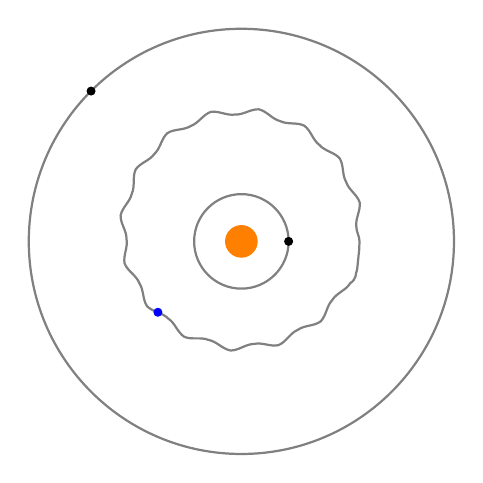
\begin{tikzpicture}[decoration={snake,amplitude=.4mm,segment length=6mm,post length=1mm}]
			\draw [gray,thick,radius=2.7cm] (0,0) circle;
			\draw [gray,decorate,thick,radius=1.5cm] (0,0) circle;
			\draw [gray,thick,radius=0.6cm] (0,0) circle;
			\filldraw [draw=orange,fill=orange,radius=0.2cm] (0,0) circle; 

			\node [shape=circle,draw=black,fill=black,inner sep=1pt] at (0.6,0) {};
			\node [shape=circle,draw=blue,fill=blue,inner sep=1pt] at (-1.060,-0.9) {};
			\node [shape=circle,draw=black,fill=black,inner sep=1pt] at (-1.909,1.909) {};
		\end{tikzpicture}
		&
		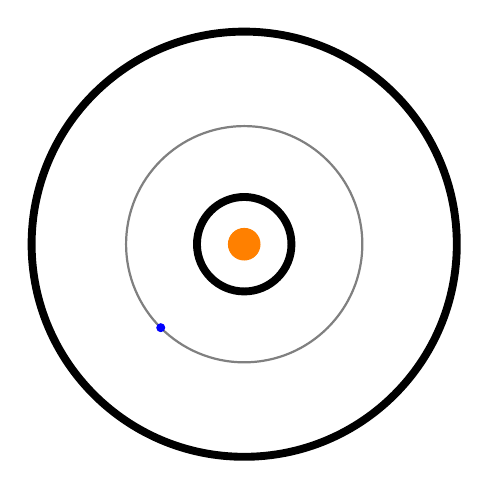
\begin{tikzpicture}[decoration={snake,amplitude=.4mm,segment length=6mm,post length=1mm}]
			\draw [line width=0.1cm,radius=2.7cm] (0,0) circle;
			\draw [gray,thick,radius=1.5cm] (0,0) circle;
			\draw [line width=0.1cm,radius=0.6cm] (0,0) circle;
			\filldraw [draw=orange,fill=orange,radius=0.2cm] (0,0) circle; 

			\node [shape=circle,draw=blue,fill=blue,inner sep=1pt] at (-1.060,-1.060) {};
		\end{tikzpicture} \\
		reales Planetensystem & Hartree-Fock-Planetensystem
		\end{tabular}
	\caption{\HF and real planetary system}
	\label{fig:HFplanets}
\end{figure}


% effective one-particle problem
%	-> show picture of cloud of interactions
%	-> show planetary system picture
% averaged interactions
% show dsa pictures



%still a good ansatz
\begin{itemize}
\item
$\psi$ HF orbitals or (SCF) orbital basis,
typically in FCI one uses the HF orbital basis as the one-particle basis functions for FCI
	\end{itemize}


\todo[inline,caption={}]{
	\begin{itemize}
		\item What is it and where does HF fail
		\item A couple of sentences about truncated CI
			\begin{itemize}
				\item Brief explanation what
				\item Mention size-consistency issues
			\end{itemize}
	\end{itemize}
}

Correlation energy: Difference HF to FCI
(even though HF not fully uncorrelated)

dynamic vs. static correlation


We will discuss so-called \newterm{truncated CI methods},
which only include determinants up to a certain
degree of excitations (double, triple, quadruple, \ldots)
in the context of so-called correlation methods in \vref{sec:Correlation}.


\subsection{Second order Møller-Plesset perturbation theory}
\label{sec:MP}

% reference C. Møller, M. S. Plesset, Phys. Rev. 1934, 46, 618.


Follows Rayleigh-Schrödinger PT
introduce 0-th order and perturbation operator
state RS MP2 energy result
show final expression without derivation
introduce $T_2$ amplitude.

\begin{align*}
	\Op{H}_0 &= \sum_i \Op{F}(i) && \text{Sum of Fock operators} \\
	\Op{V} &= \Op{H} - \Op{H}_0 = \sum_{i<j} \frac{1}{r_{ij}} - \sum_i \Op{V}_H(i) - \sum_i \Op{V}_x(i) && \text{Perturbation operator}
\end{align*}
with
\begin{align*}
	&\Op{F}(i) && \text{Fock operator for electron $i$} \\
	&\Op{V}_H(i) && \text{Hartree potential operator for electron $i$} \\
	&\Op{V}_x(i) && \text{Exchange potential operator for electron $i$} \\
\end{align*}
one gets for the MP2 energy
\begin{align*}
	E_\text{MP2} = \sum_\tau \frac{ \abs{ \bra{\Psi_\text{HF}} \Op{V} \ket{\op{\tau} \Psi_\text{HF}} }^2 }
	{ E_0 - \bra{\Psi_\text{HF}\op{\tau}^\dagger } \Op{H}_0 \op{\tau} \ket{\Psi_\text{HF}}}
\end{align*}
where $\tau$ runs over all possible excitation operators and
\[
	E_0 = \sum_{i \in Occ} \varepsilon_i 
\]

unrestricted
\[ E_\text{MP2} = \frac14 \sum_{\substack{i,j \in Occ \\ a,b \in Virt}}
	\frac{\abs{ \eriMu{ia}{jb} - \eriMu{ja}{ib}}^2 }
	{ \varepsilon_i + \varepsilon_j - \varepsilon_a - \varepsilon_b} \]


\subsection{Coupled-cluster theory}
\defineabbr{CC}{CC\xspace}{Coupled cluster}
\label{sec:CC}

Without going into too many details
the coupled-cluster ansatz generates a wavefuction from the reference
determinant $\Phi_0$ using the exponential ansatz
\[ \Psi_\text{CC} = \exp(\op{T}) \Phi_0 \]
where
\[ \op{T} = \sum_\mu t_\mu \op{\tau}_\mu \]
Variational ansatz leads to full CI.
Instead insert ansatz into electronic Schrödinger equation
\[ \Op{H}_{\Nelec} \exp(\op{T}) \Phi_0 = E_0 \exp(\op{T}) \Phi_0 \]
Introduce similarity-transformed Hamiltonian
\[ \Op{H}_T = \exp(-\op{T}) \Op{H}_{\Nelec} \exp(\op{T}) \]
to write
\begin{align*}
	\mbra{\Phi_0} \Op{H}_T \mket{\Phi_0} &= E \\
	\mbra{\Phi_\mu} \Op{H}_T \mket{\Phi_0} &= 0
\end{align*}
where
\[ \Phi_\mu = \op{\tau} \Phi_0 \]
Projection ansatz not exact.
Number of projections equals number of excitations to consider.

size-extensive and size-consistent treatment

Consider special case of CCD
where $\op{T} = \op{T}_2 = $ doubles only.



$T_2$ amplitudes $t_{ij}^{ab}$
% adapt ccd example of molsturm to this

\defineabbr{CCD}{CCD\xspace}{Coupled cluster doubles}

Working equations
\begin{equation}
\begin{aligned}
	r_{ij}^{ab}
		&= \eriAsym{ab}{ij} \\
		%
		&+ \sum_e f_{ae} \, t_{ij}^{eb}
		 - \sum_e f_{be} \, t_{ij}^{ea}
		 - \sum_m f_{mi} \, t_{mj}^{ab}
		 + \sum_m f_{mj} \, t_{mi}^{ab} \\
		%
		&+ \frac12 \sum_{mn} \eriAsym{mn}{ij} \, t_{mn}^{ab}
		+ \frac12 \sum_{ef} \eriAsym{ab}{ef} \, t_{ij}^{ef} \\
		%
		&+ \sum_{me} \eriAsym{mb}{ej} \, t_{im}^{ae}
		 - \sum_{me} \eriAsym{mb}{ei} \, t_{jm}^{ae} \\
		&- \sum_{me} \eriAsym{ma}{ej} \, t_{im}^{be}
		 + \sum_{me} \eriAsym{ma}{ei} \, t_{jm}^{be} \\
		%
		&- \frac12 \sum_{mnef} \eriAsym{mn}{ef} \, t_{mn}^{af} \, t_{ij}^{eb}
		 + \frac12 \sum_{mnef} \eriAsym{mn}{ef} \, t_{mn}^{bf} \, t_{ij}^{ea} \\
		&- \frac12 \sum_{mnef} \eriAsym{mn}{ef} \, t_{in}^{ef} \, t_{mj}^{ab}
		 + \frac12 \sum_{mnef} \eriAsym{mn}{ef} \, t_{jn}^{ef} \, t_{mi}^{ab} \\
		&+ \frac14 \sum_{mnef} \eriAsym{mn}{ef} \, t_{mn}^{ab} \, t_{ij}^{ef}
		 + \frac12 \sum_{mnef} \eriAsym{mn}{ef} \, t_{im}^{ae} \, t_{jn}^{bf} \\
		&- \frac12 \sum_{mnef} \eriAsym{mn}{ef} \, t_{jm}^{ae} \, t_{in}^{bf}
		 - \frac12 \sum_{mnef} \eriAsym{mn}{ef} \, t_{im}^{be} \, t_{jn}^{af} \\
		&+ \frac12 \sum_{mnef} \eriAsym{mn}{ef} \, t_{jm}^{be} \, t_{in}^{af}
\end{aligned}
	\label{eqn:CCDworking}
\end{equation}
expain terms

see original paper \cite{Bartlett1978}
or detailed derivation \cite{Hodecker2016}


\begin{equation}
	E_\text{CCD} = \frac14 \sum_{ijab} \eriAsym{ij}{ab} t_{ij}^{ab}
	\label{eqn:CCDenergy}
\end{equation}


\defineabbr{ADC}{ADC\xspace}{Algebraic-diagramatic construction}
\subsection{Excited states methods}
Drop names no details
eom-CC
lr-CC
adc

\section{Density-functional theory}
\label{sec:DFT}
In this section we want to briefly look at a different
approach towards modelling the electronic structure.
Instead of solving for the wave function $\Psi_0$ associated to the
ground state of the electronic Hamiltonian $\Op{H}_{\Nelec}$,
the idea behind \newterm{density-functional theory}
is to solve for the state's electronic density $\rho_0$ instead.

The rationale for this is twofold.
Firstly the density contains all information about the chemical system.
The integral
$\int_{\R^3} \rho(\vec{r}) \D\vec{r}$
evaluates to the number of electrons $\Nelec$
and via Kato's cusp condition~\cite{Kato1951} one may obtain the nuclear
charges $Z_A$ via the derivatives of the electron density at the cusp points.
Secondly the Hohnberg-Kohn theorems~\cite{Hohenberg1964}
as well as the Levy constrained search ansatz~\cite{Levy1979}
provide a unique identification between a particular ground state electron density
and the potential, which generates this density.
Even from a mathematical point of view
solving for the ground state density $\rho_0(\vec{r})$ is thus
sufficient to characterise all properties of the ground state of a system.

The Levy constrained search ansatz~\cite{Levy1979}
provides a conceptionally rather
intuitive route to obtain the ground state density,
namely by a constrained minimisation of the energy
with respect to all possible densities.
The issue with this procedure is that a closed-form expression
for the energy functional $\mathcal{E}(\rho)$,
which returns the energy of a given density,
is not known for any relevant chemical system.
In other words Levy constrained search in the form presented so far
cannot be applied to chemical systems.

Further progress can be made with the Kohn-Sham ansatz~\cite{Kohn1965}, however.
The idea is to consider a fictitious system of
$\Nelec$ non-interacting electrons,
which still has the property that it reproduces the exact
ground state density of the full, interacting system.
Ignoring spin in our discussion,
in this model system the exact wave function is a single determinant
\begin{align*}
	\Psi &= \Phi_\Theta = \bigwedge_{i=1}^{\Nelec} \psi_i
	&&\text{where}&
	\Theta \equiv \left(\psi_1, \psi_2, \ldots, \psi_{\Nelec}\right)
	&\in \left(H^1(\R^3, \C)\right)^{\Nelec}
\end{align*}
is a tuple of $\Nelec$ single-particle functions.
Ignoring spin the resulting ground state density is
\[
	\rho_\Theta(\vec{r}) = \sum_{i=1}^{\Nelec} \abs{\psi_i(\vec{r})}^2,
\]
which allows to write the Kohn-Sham energy functional as
\begin{equation}
	\begin{aligned}
	\mathcal{E}^\text{KS}(\Theta)
	&= \frac12 \sum_{i=1}^{\Nelec} \int_{\R^3} \norm{\nabla \psi_i}_2^2 \D\vec{r}
	+ \int_{\R^3} \sum_{A=1}^M
		\frac{Z_A \, \rho_\Theta(\vec{r})}{\norm{\vec{r} - \vec{R}_A}_2} \D\vec{r} \\
	&\hspace{20pt}
	+ \frac12 \int_{\R^3}\int_{\R^3}
		\frac{\rho_\Theta(\vec{r}_1) \rho_\Theta(\vec{r}_2)}
			{\norm{\vec{r}_1 - \vec{r}_2}_2} \D\vec{r}_1 \D\vec{r}_2
	+ E_{xc}(\rho_\Theta).
	\end{aligned}
	\label{eqn:KSEnergyFunctional}
\end{equation}
In this expression $E_{xc}$ is the \newterm{exchange-correlation functional},
which depends only on the density function $\rho$.
This term is supposed to describe the non-local
many-body effects not yet contained in the other terms,
which is threefold,
(1) the part of the kinetic energy missed by the non-interacting electrons,
(2) the exchange interaction as well as (3) correlation effects.
The crux with Kohn-Sham \DFT is that its exact functional form is unknown,
such that one has to live with approximations.
Which exchange-correlation functional is sensible for a particular
problem depends very much on the context of the chemical system,
the property one is interested in and is still subject of debate
in quantum-chemical literature.
Notice, however, that if the exact exchange-correlation functional was to be found,
\eqref{eqn:KSEnergyFunctional} would yield the exact ground-state energy.

Following the original Levy constrained search,
we want to find the density corresponding to the minimal energy,
which in the Kohn-Sham picture implies the minimisation
of $\mathcal{E}^\text{KS}(\Theta)$ with respect to the orbitals,
thus the problem
\begin{equation}
	E_0 \leq E_0^\text{KS}
	= \inf \left\{
		\mathcal{E}^\text{KS}(\Theta)
		\, \middle| \,
		\Theta \in \left(H^1(\R^3, \C)\right)^{\Nelec}, \,
		\forall i,j \,
		\braket{\psi_i}{\psi_j}_1 = \delta_{ij}.
	\right\}.
	\label{eqn:KSMO}
\end{equation}
Both the energy functional \eqref{eqn:KSEnergyFunctional}
as well as the Kohn-Sham minimisation problem \eqref{eqn:KSMO} are closely
related to the \HF problem \eqref{eqn:HFMO}.
In fact the only difference is the substitution of the exchange energy term
by the exchange-correlation functional.
As such it should not be very surprising that the methods employed to solve
\eqref{eqn:KSMO} are very similar to \HF as well.
The conditions to obtain the stationary points of \eqref{eqn:KSMO},
the Euler-Lagrange equations,
can be reformulated as
\begin{align}
	\label{eqn:KSequations}
	\Op{F}^\text{KS}_{\Theta^0} \psi_i^0 &= \varepsilon_i \psi_i^0
	&&\text{and}&
	\braket{\psi_i^0}{\psi_j^0} &= \delta_{ij}
\end{align}
where $\Theta^0$ is the minimiser of \eqref{eqn:KSMO} and
\begin{equation}
	\Op{F}_{\Theta^0}^\text{KS} = \Op{T} + \Op{V}_0 + \Op{J}_{\Theta^0} + V_{xc}
	\label{eqn:KohnShamOperator}
\end{equation}
is the Kohn-Sham operator.
Its difference to the Fock operator \eqref{eqn:FockOperator}
is again simply the replacement of the exchange operator $\op{K}_{\Theta^0}$
by the \newterm{exchange-correlation potential} $V_{xc}(\vec{r})$,
which is the derivative of the exchange-correlation energy $E_{xc}(\rho)$
with respect to the density function $\rho$.
Equation \eqref{eqn:KSequations} as well as the minimisation problem
\eqref{eqn:KSMO} can now be discretised
similar to the procedure outlined in section \vref{sec:DiscreteHF}
for Hartree-Fock,
which leads to an iterative self-consistent field procedure,
which is very similar to the Hartree-Fock \SCF outlined in
remark \vref{rem:PropertiesDiscretised}.
Algorithmically both for Kohn-Sham \DFT as well as \HF the same type of problem
needs to be solved, such that all of the numerical procedures
discussed in the next chapters for \HF could be applied to Kohn-Sham \DFT
with only very few changes.

Even though the mathematical problem of the Kohn-Sham \DFT ansatz is related
to \HF, one should mention that \DFT in combination with modern
exchange-correlation functionals~%
\cite{Tsuneda2014,Grimme2011,Perdew2005,Perdew1996,Becke1993,Lee1988}
is much more exact than \HF
for common applications of quantum-chemical calculations.
Since the cost is comparable to \HF,
it has thus become by far the most widely used method of
electronic structure theory.

